\textbf{(a) Verify that the mean service time in Example 3.1.4 is 1.5.}\\
\textbf{(b) Verify that the steady-state statistics in Example 3.1.4 seem to be correct.}\\
\textbf{(c) Note that the arrival rate, service rate, and utilization are the same as those in Example 3.1.3. Explain (or conjecture) why this is so. Be Specific.}\\
\begin{center}
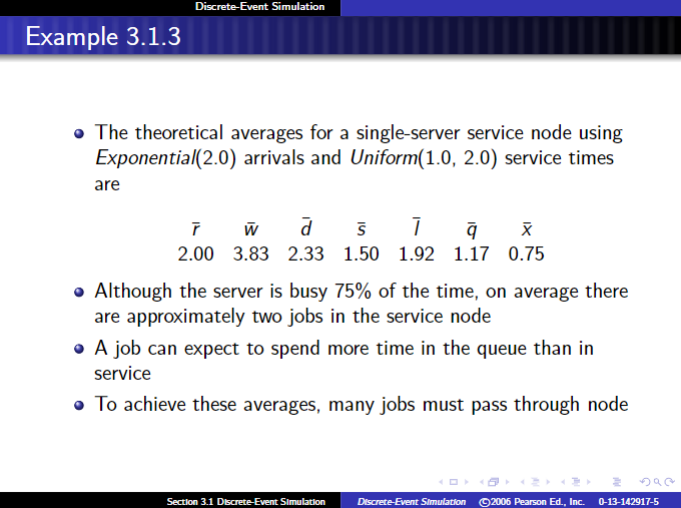
\includegraphics[scale=0.75]{Sections/Q2/3.1.3.png}\\
\vspace{10pt}
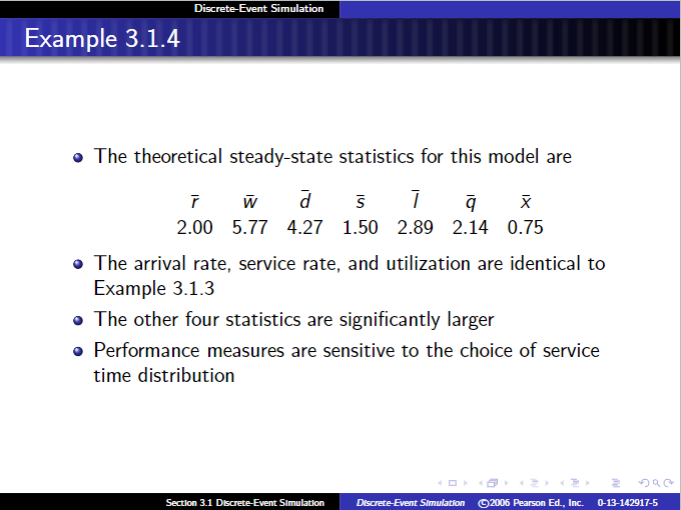
\includegraphics[scale=0.75]{Sections/Q2/3.1.4.png}\\
\end{center}
\newpage
\vspace{35pt}
\begin{center}
    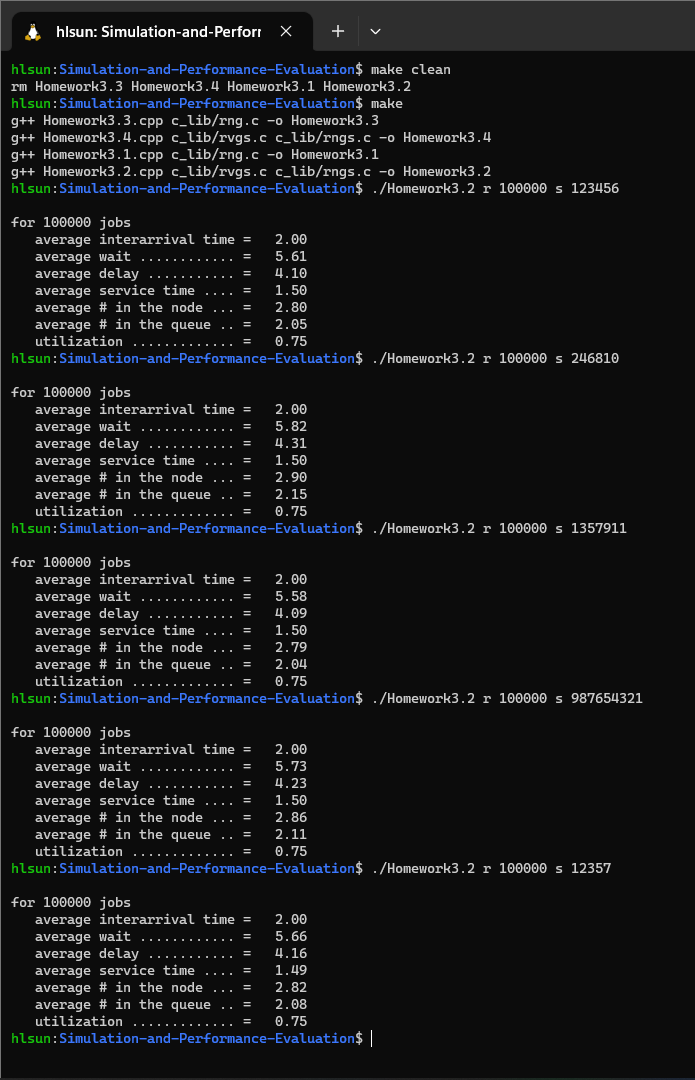
\includegraphics[scale=0.75]{Sections/Q2/H3_2.png}
\end{center}
\newpage
\begin{table}[h]
\centering
\begin{tabular}{l|lllll}
                  & 123456 & 246810 & 1357911 & 987654321 & 12357 \\
                  \hline\\
interarrival time & 2.00   & 2.00   & 2.00    & 2.00      & 2.00  \\
wait time         & 5.61   & 5.82   & 5.58    & 5.73      & 5.66  \\
delay time        & 4.10   & 4.31   & 4.09    & 4.23      & 4.16  \\
service time      & 1.50   & 1.50   & 1.50    & 1.50      & 1.49  \\
number in node    & 2.80   & 2.90   & 2.79    & 2.86      & 2.82  \\
number in queue   & 2.05   & 2.15   & 2.04    & 2.11      & 2.08  \\
utilization       & 0.75   & 0.75   & 0.75    & 0.75      & 0.75 
\end{tabular}
\end{table}
\noindent The arrival rate is the same because the interarrival time is defined by the same distribution as in Example 3.1.3: $r \sim Exponential(2.0)$.\\\\

\noindent The average service rate is the same as in Example 3.1.3 due to the distribution of the service times. The average number of tasks $\Bar{t}$ of $t \sim 1+ Geometric(0.9)$ is $1$ plus the inverse of $p=0.9$. Therefore, the average number of tasks is 10. The average of $Uniform(0.1, 0.2)$ is $0.15$. Multiplying this and the number of tasks together results in an average service rate $\Bar{s} = 1.5$, which is the same as the service rate in Example 3.1.3.\\\\

\noindent The server utilization is the same as in Example 3.1.3 because the average interarrival times and average service rates are the same in both examples. The server utilization is a ratio of the interarrival and service time averages.

\newpage
\begin{lstlisting}[style=CStyle]
/**
 * Homework 3.2
 * EECE 5643 - Simulation and Performance Evaluation
 * Author: Harrison Sun
 * Email: sun.har@northeastern.edu
 */

#include <cstdlib>
#include <cstring>
#include <stdio.h>
#include <exception>
#include <iostream>
#include <math.h> 
#include <string>
#include "c_lib/rvgs.h"
#include "c_lib/rngs.h"

#define LAST         10000L                   /* number of jobs processed */
#define START        0.0                      /* initial time             */

 /**
  * double GetArrival()
  *
  * @param void
  * @return arrival - the next arrival time
  *
  * This function calculates the arrival times for each process.
  */

double GetArrival()
{
    static double arrival = START;

    arrival += Exponential(2.0);
    return (arrival);
}


/**
 * double GetService()
 *
 * @param void
 * @return sum - the total service time for the process
 *
 * This function calculates the service times for each process.
 */

double GetService()
{
    long k{};
    double sum{ 0.0 };
    long tasks = 1 + Geometric(0.9);
    for (k = 0; k < tasks; ++k)
    {
        sum += Uniform(0.1, 0.2);
    }
    return sum;
}

/**
 * bool checkArg()
 *
 * @param char* input - the input string literal from the console
 * @return bool - true if the input is a number, false otherwise
 *
 * This function determines whether the argument is a number.
 */

bool checkArg(char* input)
{
    try
    {
        if (strlen(input) > 9)
        {
            throw std::logic_error("Number is too large.");
        }

        for (int i = 0; i < strlen(input); ++i)
        {

            if (std::isdigit(input[i])) continue;
            else
            {
                std::string errorMessage;
                errorMessage.append((std::string)input);
                errorMessage.append(" is not a digit.");
                throw std::logic_error(errorMessage);
            }
        }
        return 1;
    }

    catch (const std::logic_error& error)
    {
        std::cerr << error.what() << std::endl;
        return 0;
    }
}

/**
 * int main()
 *
 * @param int argc - the number of arguments
 * @param char* argv[] - the arguments
 *
 * @return int - 0 if the program runs successfully
 */

int main(int argc, char* argv[])
{
    long   index = 0;                         /* job index            */
    double arrival = START;                     /* time of arrival      */
    double delay;                                 /* delay in queue       */
    double service;                               /* service time         */
    double wait;                                  /* delay + service      */
    double departure = START;                     /* time of departure    */
    struct {                                      /* sum of ...           */
        double delay;                               /*   delay times        */
        double wait;                                /*   wait times         */
        double service;                             /*   service times      */
        double interarrival;                        /*   interarrival times */
    } sum = { 0.0, 0.0, 0.0 };

    long numRuns{};                                  /* number of runs */

    // Set the seed
    for (int i = 0; i < argc; ++i)
    {
        if (*argv[i] == 's' && checkArg(argv[i + 1]))
        {
            PutSeed(std::stol(argv[i + 1]));
            break;
        }
        else
        {
            PutSeed(123456789);
        }
    }

    // Set the number of runs
    for (int i = 0; i < argc; ++i)
    {
        if (*argv[i] == 'r' && checkArg(argv[i + 1]))
        {
            numRuns = std::stol(argv[i + 1]);
            break;
        }
        else
        {
            numRuns = 10000;
        }
    }

    while (index < numRuns) {
        index++;
        arrival = GetArrival();
        if (arrival < departure)
            delay = departure - arrival;         /* delay in queue    */
        else
            delay = 0.0;                         /* no delay          */
        service = GetService();
        wait = delay + service;
        departure = arrival + wait;              /* time of departure */
        sum.delay += delay;
        sum.wait += wait;
        sum.service += service;
    }
    sum.interarrival = arrival - START;

    printf("\nfor %ld jobs\n", index);
    printf("   average interarrival time = %6.2f\n", sum.interarrival / index);
    printf("   average wait ............ = %6.2f\n", sum.wait / index);
    printf("   average delay ........... = %6.2f\n", sum.delay / index);
    printf("   average service time .... = %6.2f\n", sum.service / index);
    printf("   average # in the node ... = %6.2f\n", sum.wait / departure);
    printf("   average # in the queue .. = %6.2f\n", sum.delay / departure);
    printf("   utilization ............. = %6.2f\n", sum.service / departure);
    return 0;
}
\end{lstlisting}